\documentclass[a4paper]{article}
\usepackage{graphicx}
\usepackage{hyperref}
\usepackage{amsmath}
\usepackage{amssymb}
\usepackage{textcomp}
\usepackage[utf8]{inputenc}
\usepackage[polish]{babel}
\usepackage[T1]{fontenc}
\usepackage{standalone}
\usepackage{array}
% pakiet stosowany do url'i w bibliografii, zamienia odnośniki na ładnie sformatowane
\usepackage{url}
% pakiety służące do numerowania i tworzenia algorytmów
\usepackage{algorithmic}
\usepackage{algorithm}
% redefinicja etykiety nagłówkowej listy algorytmów, domyślna jest po angielsku
\renewcommand{\listalgorithmname}{Spis algorytmów}
\addto\captionspolish{\renewcommand{\figurename}{Fig.}}
\addto\captionspolish{\renewcommand{\refname}{References}}
%\renewcommand{\bibname}{References}
% pakiet do wyliczania skali, przydatny przy dużych obrazkach
\usepackage{pgf}
% pakiet służący do automatycznego sortowania odnośników do bibliografii
\usepackage[sort]{natbib}
% tworzenie listingów
\usepackage{listings}
% tworzenie figur wewnątrz figur
\usepackage{subfig}
% do automatycznego skracania nazw rozdziałów i podrozdziałów używanych w nagłówkach strony by mieściły się w jednej linii
\usepackage[fit]{truncate}
% fancyhdr - ładne nagłówki, definicja wyglądu nagłówka, numery stron będą umieszczane w nagłówku po odpowiedniej stronie
\usepackage{fancyhdr}
\pagestyle{fancy}
%\renewcommand{\chaptermark}[1]{\markboth{#1}{}}
\renewcommand{\sectionmark}[1]{\markright{\thesection\ #1}}
\fancyhf{}
% tutaj ograniczamy szerokość pola w nagłówku zawierającego nazwę rozdziału/podrozdziału do 95% szerokości strony
% redefinicja sposobu prezentacji nazw domyślnie wypisywanych wielkimi literami (np. domyślnie w nagłówku Spis treści będzie miał postać SPIS TREŚCI)
% Uwaga! to może popsuć wielkie litery w ogóle! Jak coś nie działa należy usunąć \nouppercase{} z poniższych definicji
\fancyhead[LO]{\nouppercase{\bfseries{\truncate{.95\headwidth}{\rightmark}}}}
\fancyhead[RE]{\nouppercase{\bfseries{\truncate{.95\headwidth}{\leftmark}}}}
\renewcommand{\headrulewidth}{0.5pt}
\renewcommand{\footrulewidth}{0pt}

% definicja typu prostego wymagana przez pierwsze strony rozdziałów itp.
% powyższe reguły niestety tych stron nie dotyczą, gdyż Latex automatycznie przełącza je pomiędzy fancy a plain
% w tym wypadku eliminujemy nagłówki i stopki na stronach początkowych
\fancypagestyle{plain}{%
 \fancyhead{}
 \fancyfoot{}
 \renewcommand{\headrulewidth}{0pt}
 \renewcommand{\footrulewidth}{0pt}
}

\parskip 0.05in


% makro umożliwiające otaczanie symboli okręgami
\usepackage{tikz}
% brak justowania tekstu (bazą okręgu będzie linia tekstu)
\newcommand*\mycirc[1]{%
  \begin{tikzpicture}
    \node[draw,circle,inner sep=1pt] {#1};
  \end{tikzpicture}}

% pionowe justowanie tekstu, środek okręgu pokrywa się ze środkiem tekstu
\newcommand*\mycircalign[1]{%
  \begin{tikzpicture}[baseline=(C.base)]
    \node[draw,circle,inner sep=1pt](C) {#1};
  \end{tikzpicture}}

% zmiana nazwy twierdzeń i lematów
\newtheorem{theorem}{Twierdzenie}[section]
\newtheorem{lemma}[theorem]{Lemat}

% tworzenie definicji dowodu
\newenvironment{proof}[1][Dowód]{\begin{trivlist}
\item[\hskip \labelsep {\bfseries #1}]}{\end{trivlist}}
% \newenvironment{definition}[1][Definicja]{\begin{trivlist}
% \item[\hskip \labelsep {\bfseries #1}]}{\end{trivlist}}
% \newenvironment{example}[1][Przykład]{\begin{trivlist}
% \item[\hskip \labelsep {\bfseries #1}]}{\end{trivlist}}
% \newenvironment{remark}[1][Uwaga]{\begin{trivlist}
% \item[\hskip \labelsep {\bfseries #1}]}{\end{trivlist}}

% definicja czarnego prostokąta zwyczajowo dodawanego na koniec dowodu
\newcommand{\qed}{\nobreak \ifvmode \relax \else
      \ifdim\lastskip<1.5em \hskip-\lastskip
      \hskip1.5em plus0em minus0.5em \fi \nobreak
      \vrule height0.75em width0.5em depth0.25em\fi}

% poniższymi instrukcjami można sterować co ma być numerowane a co nie i co ma być wyświetlane w spisie treści
% \setcounter{secnumdepth}{3}
% \setcounter{tocdepth}{5}

% definicja czcionki mniejszej niż tiny (domyślnie takiej małej nie ma)
\usepackage{lmodern}
\makeatletter
  \newcommand\tinyv{\@setfontsize\tinyv{4pt}{6}}
\makeatother

% definicja jeszcze mniejszej czcionki
\usepackage{lmodern}
\makeatletter
  \newcommand\tinyvv{\@setfontsize\tinyvv{3.5pt}{6}}
\makeatother

% pakiet do obsługi wielostronicowych tabel
\usepackage{longtable}
\setlength{\LTcapwidth}{\textwidth}

\usepackage[section] {placeins}

\usepackage{multirow}

\usepackage{slantsc}



\begin{document}

\begin{flushright}
{\large \today}
\end{flushright}

\begin{center}



\textsc{\LARGE Intelligent Information Retrieval }\\[1.5cm]

\textsc{\Large Project }\\[0.5cm]

% Title
%\HRule \\[0.4cm]
{ \huge \bfseries Agent with cognitive structure \\[0.4cm] }

%\HRule \\[1.5cm]

% Author and supervisor
\end{center}
\begin{minipage}{0.7\textwidth}
\begin{flushleft} \large
\emph{Authors:}\\
inż. Mateusz Bodziak 131101 IDS, KSDiR\\
inż. Szymon Grocholski 131126 IDS, KSDiR\\

\end{flushleft}
\end{minipage}

\section{Introduction}
The project is about to implement an agent which should learn the rules of the Wumpus World game. The solution will be based on neuron networks.
	
	\subsection{Main idea}
	Our task was to create an agent without a priori knowledge about the game, the 
	environment and rules then train him and check whether he has learnt something.Main idea is to prepare a training set which will be used by a neural network to learn
	 the rules of the world and test is comparing with different network architectures.
	 Main data flow is shown in the Pic.~\ref{pic:flow}.
	 \begin{figure}[!h]
		\centering	
		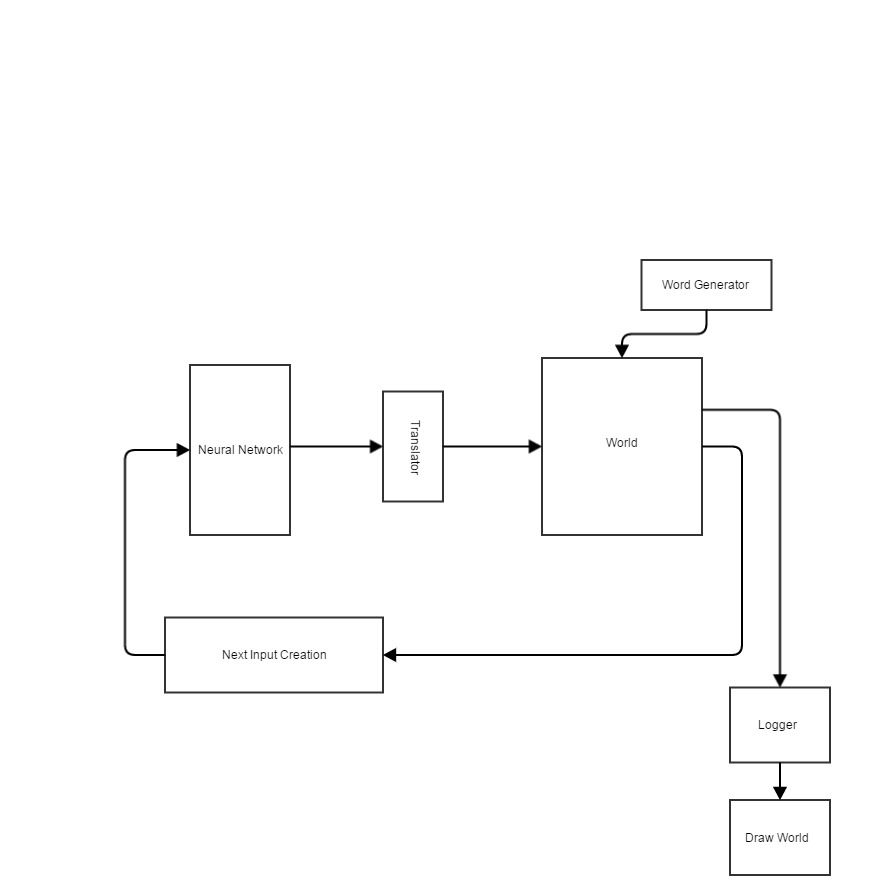
\includegraphics[width=1.2\textwidth]{pic/arch.jpg}
		\caption{Data flow of the program }
		\label{pic:flow}
	\end{figure}
	\subsection{Neural Network}
	Our neural network contains parametirized number of hidden layers in testing phase we 
	used 1 and 2 layers. The version with one layer is presented on the Pic~\ref{pic:networkExample}
	\begin{figure}[!h]
		\centering	
		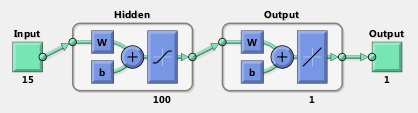
\includegraphics[width=\textwidth]{pic/networkExample.jpg}
		\caption{One of the network architectures}
		\label{pic:networkExample}
	\end{figure}
	
 The input vector is as follows:
	$$
		[x_i, y_i, senses(i), x_(i-1), y_(i-1), senses(i-1), x_(i-2), y_(i-2), senses(i-2)]
	$$
	where 
		$x_i$ - is the current position the row coordinate
		$y_i$ - is the current position the column coordinate
		$senses(i)$ - is a vector of senses from field with coordinates $(x_i, y_i)$
		rest of the coefficients are analogical from previous steps
	
	The output of the network gives us a number from $0-360$ which is the angle. This value
	is translated to a move according to the Pic.~\ref{pic:compass}
	\begin{figure}[!h]
	\centering	
	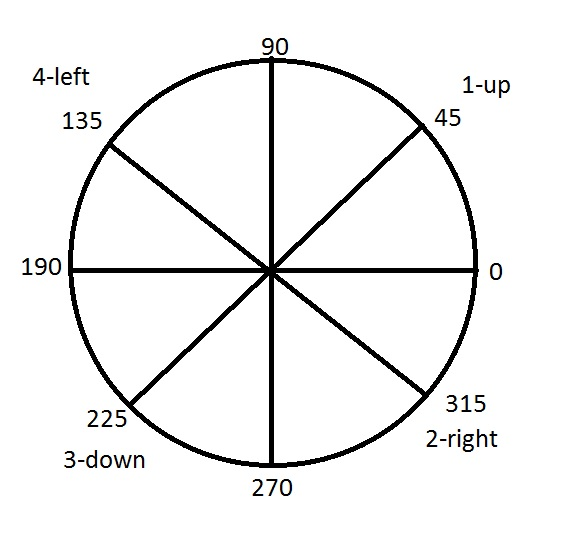
\includegraphics[width=0.7\textwidth]{pic/kompass.jpg}
	\caption{The picture shows how angles are mapped into move}
\label{pic:compass}
\end{figure}
	\begin{itemize}
		\item 1 - UP
		\item 2 - RIGHT
		\item 3 - DOWN
		\item 4 - LEFT
	\end{itemize}
	

\section{Implementation }
		\begin{enumerate}
		\item Training data preparation
			\begin{itemize}
				\item Manual data generator 
				\item Automated data generator
			\end{itemize}
		\item Network training 
		\item Execution
			\begin{itemize}
				\item Animation of one walkthrough
				\item Comparison of two networks 
			\end{itemize}
	\end{enumerate}
	
	\paragraph{Training data}
	We construct two ways of preparing the training data. First one was automated, prepared 
	based on random walkthroughs from which we select and store only good ones. This method
	 generated walkthroughs with success - gold was found. Unfortunately this method has stored 
	 many moves which had no sense, like bumping often into walls and ignoring the meaning 
	 of the senses.  
	 Improvement of this was to input some a prori knowledge by human, so we created the manual
	 training data generator which stored the walkthroughs which were committed by a real human player.
	 This enabled us to prepare more suitable training set but it was tiresome and time consuming method.
	 
	 
	\paragraph{Network training}
	In this stage we use our training date prepared in the previous stage to train the network.
	The concept of the training is presented on Pic.~\ref{pic:trainDataAuto}
	 \begin{figure}[!h]
		\centering	
		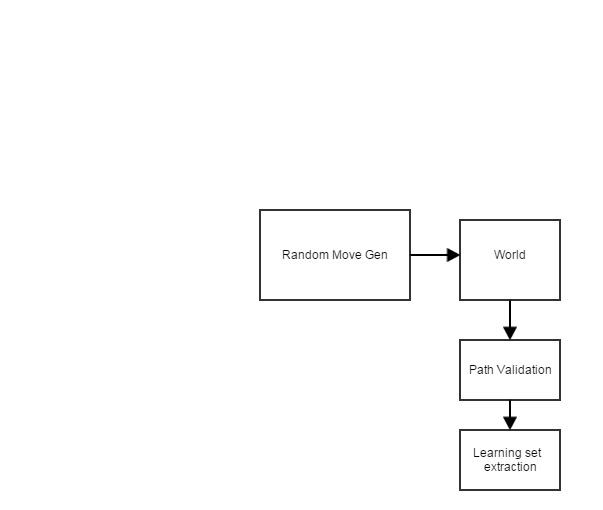
\includegraphics[width=0.7\textwidth]{pic/trainDataAuto.jpg}
		\caption{The algorithm of the training}
		\label{pic:trainDataAuto}
	\end{figure}
	\paragraph{Execution}
	
	

	





\section{Conclusions}

\end{document}
